% !TeX root = ../main.tex
% Add the above to each chapter to make compiling the PDF easier in some editors.

\chapter{Lagrange Multipliers and Duality}\label{cha:lagrange_multipliers_duality}

\section{Separating Hyperplanes}

\begin{defn}[Hyperplane] A \emph{hyperplane}\index{hyperplane} of dimension $n$ is the subset, \begin{align}
    \sH(\vn,\mu) \defeq \{\vx \in \R^n \mid \trans{\vn}\vx = \mu\},
\end{align} for some \emph{normal}\index{normal vector} $\vn \in \R^n \setminus \{\vZero\}$ and \emph{threshold} $\mu \in \R$.
\end{defn}

Every hyperplane divides $\R^n$ into two half-spaces $\{\vx \mid \trans{\vn}\vx \leq \mu\}$ and $\{\vx \mid \trans{\vn}\vx \geq \mu\}$. It separates two sets, if they lie in different half-spaces.

\begin{defn}[Separating hyperplane] We say a hyperplane $\sH$ \emph{separates}\index{separating hyperplane} two sets $\sA, \sB$ iff \begin{align}\begin{split}
    \forall a \in \sA: \trans{\vn}\va &\leq \mu \quad\text{and} \\
    \forall b \in \sB: \trans{\vn}\vb &\geq \mu.
\end{split}\end{align} If the inequalities are strict, we say that $\sH$ \emph{strictly} separates $\sA$ and $\sB$.
\end{defn}

If $\sA, \sB$ are non-convex, we are not guaranteed that a separating hyperplane exists (e.g., a point cannot be separated from a ring around it). However, if we assume that $\mA$ and $\mB$ are convex, a separating hyperplane always exists.

\begin{fct}[Separating hyperplane theorem]\index{Separating hyperplane theoerm} Given two disjoint and non-empty convex subsets $\sA, \sB \subseteq \R^n$, there exists a separating hyperplane.
\end{fct}

However, it is not true that there always exists a strictly separating hyperplane. Consider $\sA \defeq \{(x,y) \mid x \leq 0\}$ and $\sB \defeq \{(x,y) \mid x > 0 \text{ and } y \geq \frac{1}{x}\}$. Clearly they are disjoint and convex; however, the only separating hyperplane is $\sH = \{(x,y) \mid x = 0\}$, which intersects $\sA$.
\begin{marginfigure}
TBD
% \centering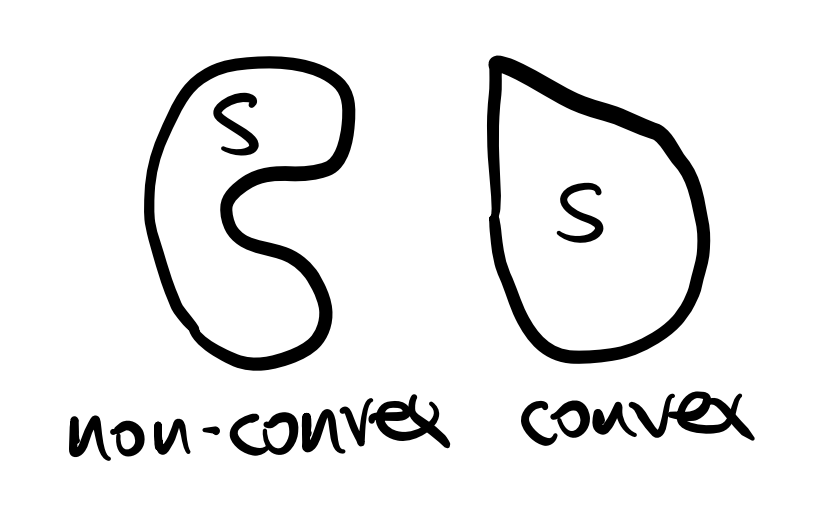
\includegraphics[width=4cm]{notes/figures/convex_set.png}
\caption{Example where no strictly separating hyperplane exists.}
\end{marginfigure}

When we also assume that $\sA$ and $\sB$ are closed and bounded, a strictly separating hyperplane always exists.

\begin{thm}[Separating hyperplane theorem; closed, bounded sets] Given two disjoint, closed, bounded, and non-empty convex subsets $\sA, \sB \subseteq \R^n$, there exists a strictly separating hyperplane.

If $\vc \in \sA, \vd \in \sB$ are minimizers of $\min_{\va \in \sA,\ \vb \in \sB} \norm{\va - \vb}_2$, then one such hyperplane is given by, \begin{align}
    \vn \defeq \vd - \vc \quad\text{and}\quad \mu \defeq \frac{1}{2}\parentheses*{\norm{\vd}_2^2 - \norm{\vc}_2^2}.
\end{align}
\begin{marginfigure}
TBD
% \centering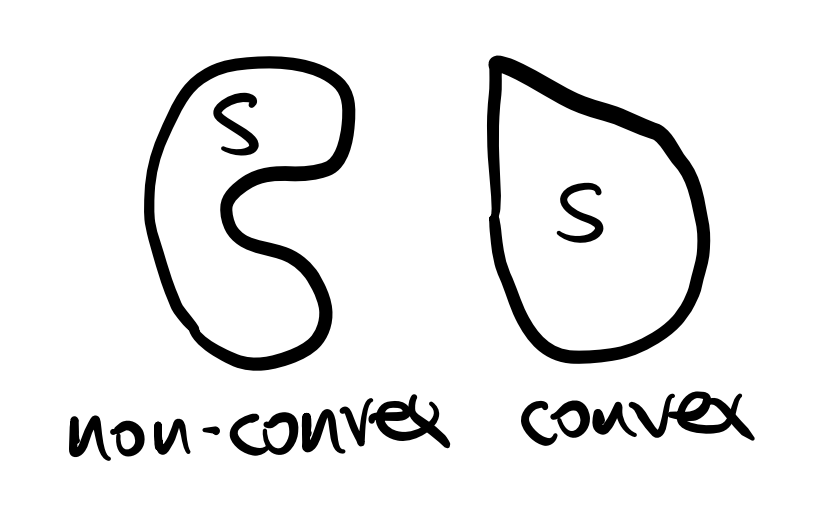
\includegraphics[width=4cm]{notes/figures/convex_set.png}
\caption{Illustration of strictly separating hyperplane.}
\end{marginfigure}
\end{thm}
\begin{proof}
We want to show that $\trans{\vn}\vb > \mu$ for all $\vb \in \sB$. Then, $\trans{\vn}\va < \mu$ for all $\va \in \sA$ follows by symmetry. We have, \begin{align*}
    \trans{\vn}\vd - \mu &= \trans{(\vd - \vc)}\vd - \frac{1}{2}\parentheses*{\norm{\vd}_2^2 - \norm{\vc}_2^2} \\
    &= \norm{\vd}_2^2 - \trans{\vd}\vc - \frac{1}{2}\norm{\vd}_2^2 + \frac{1}{2}\norm{\vc}_2^2 \\
    &= \frac{1}{2}\norm{\vd - \vc}_2^2 > 0. \margintag{using the asusmption that $\sA,\sB$ are disjoint, close, and bounded, their distance is positive}
\end{align*} Suppose for a contradiction that there exists a $\vu \in \sB$ such that $\trans{\vn}\vu - \mu \leq 0$.

Consider the line defined by the distance minimizer $\vd$ and the point on the ``wrong side'' $\vu$, $\vb(\lambda) \defeq \vd + \lambda(\vu - \vd)$. Taking the derivative of the distance between $\vb(\lambda)$ and $\vc$ and evaluating it at $\lambda = 0$ (which is when $\vb(\lambda) = \vd$), we obtain, \begin{align*}
    \left.\odv{}{\lambda}\norm{\vb(\lambda)-\vc}_2^2\right\vert_{\lambda=0} &= \left.2 \trans{(\vd - \lambda\vd + \lambda\vu - \vc)}(\vu-\vd)\right\vert_{\lambda=0} \\
    &= 2 \trans{(\vd - \vc)}(\vu - \vd).
\end{align*} However, \begin{align*}
    \trans{\vn}\vu - \mu = \trans{(\vd - \vc)}(\vu - \vd) + \underbrace{\trans{\vn}\vd - \mu}_{>0} \leq 0,
\end{align*} implies that $\trans{(\vd - \vc)}(\vu - \vd)$, and hence, the gradient are negative, which contradicts the minimality of $\vd$.
\end{proof}

\section{Lagrange Multipliers and KKT Conditions}

We will now discuss how we can treat constraints in a convex optimization problem, \begin{align}
    \s{\alpha} \defeq \min_{\substack{\vy \in \R^n \\ \mA\vy = \vb \\ \vg(\vy) \leq \vZero}} f(\vy),
\end{align} where $f : \R^n \to \R$ is convex, $\mA \in \R^{m \times n}$, $\vb \in \R^m$, and we have $k$ convex constraints $g_i : \R^n \to \R$.

\begin{rmk}
The linear constraints $\mA\vy = \vb$ are not necessary, as they can also be modeled using the (convex) constraints $\mA\vy - \vb \leq \vZero$ and $\vb - \mA\vy \leq 0$. We include them here to see later that programs with only linear constraints can be handled in a slightly different way.
\end{rmk}

We call this optimization problem the \emph{primal program}\index{primal program} and we will later see that it has an associated dual problem. We say that $\vy \in \R^n$ is \emph{primal feasible}\index{primal feasible} iff $\mA\vy = \vb$ and $\vg(\vy) \leq \vZero$.

\subsection{An Intuition}

\begin{marginfigure}
TBD
% \centering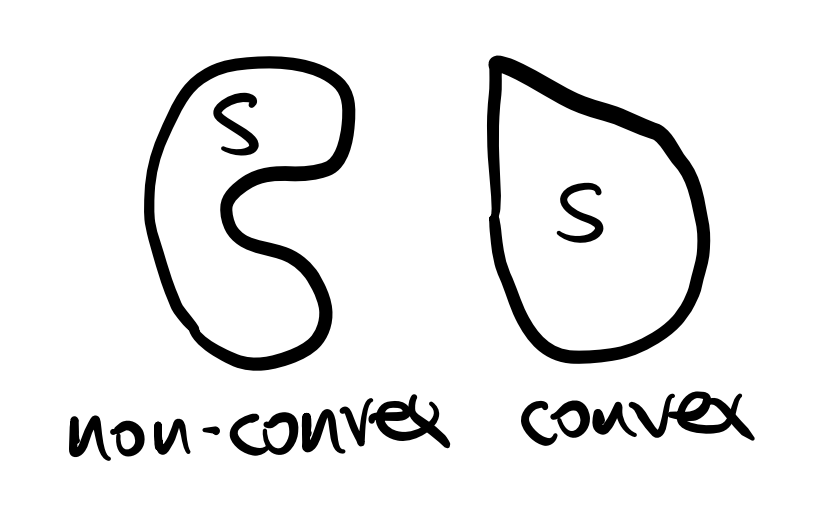
\includegraphics[width=4cm]{notes/figures/convex_set.png}
\caption{Illustration of simple constrained optimization.}
\end{marginfigure}
In the following, we want to answer the question: ``When is a feasible point optimal?'' To simplify things a bit, let us consider the optimization problem of minimizing $f$ under the single constraint $g$. Suppose we know the feasible optimum $\s{\vy}$. Then for infinitesimal $\vdelta$, if $\vdelta \perp \grad g(\s{\vy})$, then $\s{\vy} + \vdelta$ and $\s{\vy} - \vdelta$ are feasible. But then we must have that $\vdelta \perp \grad f(\s{\vy})$, or else one direction would improve the objective. This tells us that, \begin{align*}
    \trans{\vdelta}\grad f(\s{\vy}) = 0 = \trans{\vdelta}\grad g(\s{\vy}),
\end{align*} and hence, there exists some $\lambda \in \R$ such that $\grad f(\s{\vy}) = \lambda \grad g(\s{\vy})$. This is the fundamental intuition behind a \emph{Lagrange multiplier}: the gradient of the objective at an optimal point is a linear combination of the gradients of the (tight) constraints.

We say that the constraint $g_i$ is \emph{tight}\index{tight constraint} at $\vy$ iff $g_i(\vy) = 0$. We know that if $\vy$ is feasible, then $\vy + \vdelta$ is feasible for some infinitesimal $\vdelta$ if for all constraints $i \in [k]$ we have that either the constraint is not tight, $g_i(\vy) < 0$, or $\vy + \vdelta$ is ``more'' feasible, $\trans{\vdelta} \grad g_i(\vy) \leq 0$. The last condition tells us that for each tight constraint $g_i$, we get a half-space of feasible directions.
\begin{marginfigure}
TBD
% \centering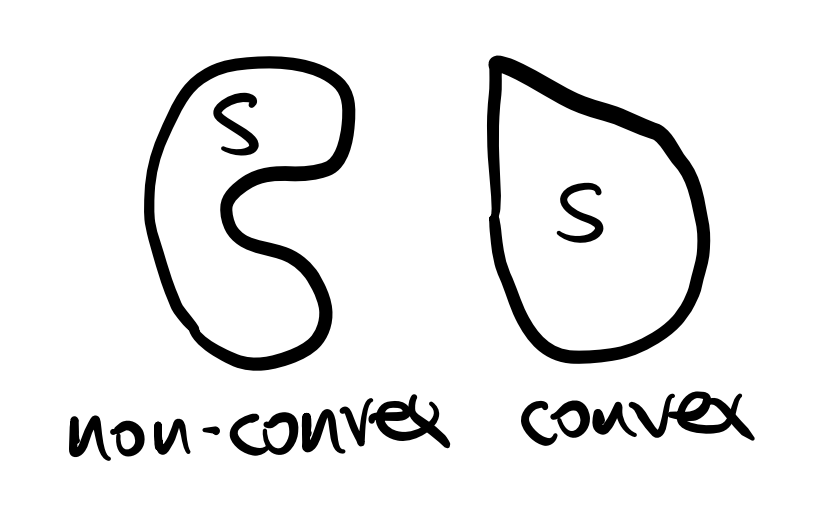
\includegraphics[width=4cm]{notes/figures/convex_set.png}
\caption{Each tight constraint yields a half-space of feasible directions.}
\end{marginfigure}

On the other hand, if $\s{\vy} + \vdelta$ is feasible, then the objective $f$ must ``worsen'', $\trans{\vdelta}\grad f(\s{\vy}) \geq 0$.

We can therefore write the gradient of $f$ at $\s{\vy}$ as a linear combination of the gradients of tight constraints.\footnote{Note that linear constraints are always tight.} Therefore, for some $\vx \in \R^m$ and $\vs \in \R^k$ with $\vs(i) \geq 0$ if $g_i(\s{\vy}) = 0$ and $\vs(i) = 0$ otherwise, \begin{align}
    - \grad f(\s{\vy}) = \sum_{i=1}^k \vs(i) \grad g_i(\s{\vy}) + \sum_{j=1}^m \vx(j) \mA(j,:). \label{eq:kkt_intro}
\end{align} The variables $\vs$ and $\vx$ are called the \emph{dual variables}\index{dual variables} and are said to be \emph{dual feasible}\index{dual feasible} iff $\vs \geq \vZero$. If $\vy$ is also primal feasible, we say that $(\vy, \vx, \vs)$ are \emph{primal-dual feasible}\index{primal-dual feasible}. \Cref{eq:kkt_intro} is equivalent to \begin{align}
    \grad f(\s{\vy}) + \trans{\grad g(\s{\vy})}\vs + \trans{\mA}\vx = \vZero \label{eq:kkt_intro2}
\end{align} along with the condition $\trans{\vg(\s{\vy})}\vs = \vZero$, ensuring that $\vs(i) = 0$ when constraint $g_i$ is not tight.

\begin{defn}[Karush-Kuhn-Tucker (KKT) conditions and Lagrangian] Points $\vy \in \R^n, \vx \in \R^m, \vs \in \R^k$ satisfy the \emph{Karush-Kuhn-Tucker conditions}\index{Karush-Kuhn-Tucker conditions} iff, \begin{align}
    \grad_\vy L(\vy, \vx, \vs) = \vZero &&\text{\emph{gradient condition}\index{gradient condition}} \\
    \trans{\vg(\vy)}\vs = \vZero &&\text{\emph{complementary slackness}\index{complementary slackness}}\margintag{ensures that $\vs(i)$ is forced to $0$ when constraint $g_i$ is not tight} \\
    \vg(\vy) \leq \vZero \quad\text{and}\quad \mA\vy = \vb &&\text{primal feasibility} \\
    \vs \geq \vZero &&\text{dual feasibility},
\end{align} where \begin{align}
    L(\vy, \vx, \vs) \defeq f(\vy) + \trans{\vs}\vg(\vy) + \trans{\vx}(\vb - \mA\vy)
\end{align} is the \emph{Lagrangian}\index{Lagrangian} of the optimization problem.
\end{defn}
\begin{rmk}
Note that, \begin{align*}
    \grad_\vy L(\vy, \vx, \vs) = \grad f(\vy) + \trans{\grad g(\vy)}\vs + \trans{\mA}\vx,
\end{align*} which coincides with our intuition from \cref{eq:kkt_intro2}.
\end{rmk}

Intuitively, if $(\vy, \vx, \vs)$ satisfy the KKT conditions, then $\vy$ is optimal. It turns out that this intuition is correct, and we will prove this in the following section.

\section{Lagrangian Duality}

We have that if $(\vy, \vx, \vs)$ are primal-dual feasible, \begin{align}
    L(\vy, \vx, \vs) = f(\vy) + \underbrace{\trans{\vs}}_{\geq \vZero}\underbrace{\vg(\vy)}_{\leq \vZero} + \trans{\vx}(\underbrace{\vb - \mA\vy}_{\vZero}) \leq f(\vy).
\end{align} We can also write the primal problem as a two-player game in terms of the Lagrangian, \begin{align}
    \s{\alpha} = \min_{\substack{\vy \in \R^n \\ \mA\vy = \vb \\ \vg(\vy) \leq \vZero}} f(\vy) = \min_{\vy \in \R^n} \max_{\substack{\vx \in \R^m \\ \vs \in \R^k \\ \vs \geq \vZero}} L(\vy, \vx, \vs).
\end{align} This is because for a minimizing $\vy$ all constraints have to be satisfied and the Lagrangian simplifies to $L(\vy, \vx, \vs) = f(\vy)$. If $\vb - \mA\vy = \vZero$ was violated, making $\vx$ large sends $L(\vy, \vx, \vs) \to \infty$. If $\vg(\vy) \leq \vZero$ was violated, making $\vs$ large sends $L(\vy, \vx, \vs) \to \infty$.

We therefore have for any dual feasible $(\vx, \vs)$, \begin{align}
    \s{\alpha} = f(\s{\vy}) \geq L(\s{\vy}, \vx, \vs) \geq \min_{\vy \in \R^n} L(\vy, \vx, \vs) \eqdef L(\vx, \vs). \label{eq:weak_duality}
\end{align}

\begin{defn}[Dual program] The \emph{dual program}\index{dual program} is given as, \begin{align}
    \s{\beta} \defeq \max_{\substack{\vx \in \R^m \\ \vs \in \R^k \\ \vs \geq \vZero}} L(\vx, \vs) = \max_{\substack{\vx \in \R^m \\ \vs \in \R^k \\ \vs \geq \vZero}} \min_{\vy \in \R^n} L(\vy, \vx, \vs).
\end{align}
\end{defn}
\begin{thm}[Weak duality]\index{weak duality}
$\s{\beta} \leq \s{\alpha}$.
\end{thm}
\begin{proof}
This follows immediately from \cref{eq:weak_duality}.
\end{proof}
\begin{rmk}
Observe that the dual program is a convex optimization problem in disguise. We can equivalently consider the optimization problem, \begin{align}
    -\s{\beta} = \min_{\substack{\vx \in \R^m \\ \vs \in \R^k \\ \vs \geq \vZero}} - L(\vx, \vs) = \min_{\substack{\vx \in \R^m \\ \vs \in \R^k \\ \vs \geq \vZero}} \max_{\vy \in \R^n} - L(\vy, \vx, \vs).
\end{align} Note that $-L(\vy, \vx, \vs)$ is a linear function in the dual variables, hence convex, and $-L(\vx, \vs)$ is a maximum of these functions, so also convex.
\end{rmk}

\begin{defn}[Strong duality] If $\s{\alpha} = \s{\beta}$, we say that \emph{strong duality}\index{strong duality} holds.
\end{defn}
\begin{rmk}
It is immediately clear that if we consider linear programs, that is, we have only linear constraints, strong duality always holds. This is because at any primal-dual feasible point $(\vy, \vx)$, we have that by definition $L(\vy, \vx) = f(\vy)$.
\end{rmk}

Before we analyze when strong duality holds, let us return to the KKT conditions and confirm our intuition from the previous section.

\begin{thm}[KKT conditions are necessary]
If strong duality holds, then the KKT conditions hold for primal-dual optimal $(\s{\vy}, \s{\vx}, \s{\vs})$.
\end{thm}
\begin{proof}
By strong duality, \begin{align*}
    L(\s{\vy}, \s{\vx}, \s{\vs}) = \s{\alpha} = \s{\beta}.
\end{align*} As $L(\vy, \s{\vx}, \s{\vs})$ is a convex function in $\vy$, we have that \begin{align*}
    \left.\grad_\vy L(\vy, \s{\vx}, \s{\vs})\right\vert_{\vy = \s{\vy}} = \vZero,
\end{align*} so the gradient condition is satisfied. Moreover, we have, \begin{align*}
    f(\s{\vy}) = \s{\alpha} = L(\s{\vy}, \s{\vx}, \s{\vs}) = f(\s{\vy}) + \trans{\vs}\vg(\s{\vy}) + \trans{\vx}(\underbrace{\vb - \mA\vy}_{\vZero}),
\end{align*} so $\trans{\vs}\vg(\s{\vy}) = \vZero$ (complementary slack) holds. By assumption, $(\s{\vy}, \s{\vx}, \s{\vs})$ are primal-dual feasible.
\end{proof}

\begin{thm}[KKT conditions are sufficient]
If the KKT conditions hold at $(\hat{\vy}, \hat{\vx}, \hat{\vs})$, then they are primal-dual optimal and strong duality holds.
\end{thm}
\begin{proof}
Because $L(\vy, \hat{\vx}, \hat{\vs})$ is a convex function, by the gradient condition, $\hat{\vy}$ is its global minimizer. Therefore, \begin{align*}
    L(\hat{\vy}, \hat{\vx}, \hat{\vs}) = \min_{\vy \in \R^n} L(\vy, \hat{\vx}, \hat{\vs}) = L(\hat{\vx}, \hat{\vs}) \leq \s{\beta}.
\end{align*} At the same time, using primal-dual feasibility and complementary slack, \begin{align*}
    L(\hat{\vy}, \hat{\vx}, \hat{\vs}) = f(\hat{\vy}) + \underbrace{\trans{\hat{\vs}}\vg(\hat{\vy})}_{\vZero} + \trans{\hat{\vx}}(\underbrace{\vb - \mA\hat{\vy}}_{\vZero}) = f(\hat{\vy}) \geq \s{\alpha}.
\end{align*} Therefore, $\s{\alpha} \leq \s{\beta}$. By weak duality, we get the opposite inequality, and hence strong duality holds.
\end{proof}

\section{Slater's Condition}

We will now discuss under which circumstances strong duality holds. In general, we can have that strong duality does not hold. \begin{ex} TBD
\end{ex}

\begin{defn}[Slater's condition] \emph{Slater's condition}\index{Slater's condition} is satisfied iff there exists some $\vy \in \R^n$ such that $\mA\vy = \vb$ and $\vg(\vy) < \vZero$.\footnote{This is satisfied by most useful optimization problems.} We say that $\vy$ is \emph{strictly feasible}\index{strictly feasible}.
\end{defn}

\begin{thm}
If Slater's condition holds, then strong duality holds.
\end{thm}
\begin{proof}
TBD
\end{proof}

\section{Example: Duality of Maximum Flow and Minimum Cut}\label{sec:max_flow_min_cut_duality}

We can write the (directed) maximum flow problem in a graph $G$ as, \begin{align}
    \max_{\substack{F \in \R \\ \vf \in \R^{|\sE|} \\ \mB\vf = F(\vOne_t - \vOne_s) \\ \vZero \leq \vf \leq \vc}} F = - \min_{\substack{F \in \R \\ \vf \in \R^{|\sE|} \\ \mB\vf = F(\vOne_t - \vOne_s) \\ \vZero \leq \vf \leq \vc}} -F.
\end{align} Here, $\vZero \leq \vf$ ensures that directions are respected, and $\vf \leq \vc$ ensures that edge capacities are respected. $F(\vOne_t - \vOne_s)$ is the demand of a flow routing $F$ units from $t$ to $s$. Observe that when there exists an $s$-$t$ path, then there are flows $\vf$ strictly satisfying the constraint $\vZero \leq \vf \leq \vc$, and hence, Slater's criterion is satisfied. By strong duality, the above program is equivalent to its dual program, \begin{align}
    &- \max_{\substack{\vx \in \R^{|\sV|} \\ \vs \in \R^{|\sE|} \\ \vs \geq \vZero}} \min_{\substack{F \in \R \\ \vf \in \R^{|\sE|} \\ \vf \geq \vZero}} -F + \trans{\vs}(\vf - \vc) + \trans{\vx}(F(\vOne_t - \vOne_s) - \mB\vf) \\
    &= \min_{\substack{\vx \in \R^{|\sV|} \\ \vs \in \R^{|\sE|} \\ \vs \geq \vZero \\ \trans{(\vOne_t - \vOne_s)}\vx = 1 \\ \vs \geq \trans{\mB}\vx}} \trans{\vs}\vc \\
    &= \min_{\substack{\vx \in \R^{|\sV|} \\ \trans{(\vOne_t - \vOne_s)}\vx = 1}} \sum_{e \in \sE} \max\{(\trans{\mB}\vx)(e), 0\}\cdot\vc(e).
\end{align} Observe that the dual program is a linear program computing the minimum cut.

\section{Fenchel Conjugates}

\begin{defn}[Fenchel conjugate]
Given a function $f : \sS \to \R$, its \emph{Fenchel conjugate}\index{Fenchel conjugate} is the function $\s{f} : \R^n \to \R$,\footnote{In principle, $\s{f}$ is a function defined over the dual space of $\sS$, but this will not be very important to us.} \begin{align}
    \s{f}(\vz) \defeq \sup_{\vy \in \sS} \trans{\vz}\vy - f(\vy).
\end{align}
\end{defn}
\begin{rmk}
$\s{f}$ is convex, as it is the maximum of linear functions.
\end{rmk}

\begin{ex}
Let us consider the function $f(\vy) \defeq \norm{\vy}$. Then we have, \begin{align}
    \s{f}(\vz) &= \sup_{\vy \in \R^n} \trans{\vz}\vy - \underbrace{\norm{\vy}}_{\eqdef \theta} \margintag{Recall that \begin{align*}
        \theta \norm{\vz}_* = \max_{\substack{\vy \in \R^n \\ \norm{\vy} = \theta}} \trans{\vz}\vy.
    \end{align*}} \nonumber\\
    &= \sup_{\theta \geq 0} \theta(\norm{\vz}_* - 1) \nonumber\\
    &= \begin{cases}
        \infty & \norm{\vz}_* > 1 \\
        0 & \text{otherwise}.
    \end{cases}
\end{align}
\end{ex}

\begin{ex}
For the function $f(\vy) \defeq \frac{1}{p} \norm{\vy}_p^p$, we have that $\s{f}(\vz) = \frac{1}{q} \norm{\vz}_q^q$, where $\frac{1}{p} + \frac{1}{q} = 1$.
\end{ex}

\begin{ex}
When we have a primal program with only linear constraints, \begin{align*}
    \min_{\substack{\vy \in \R^n \\ \mA\vy = \vb}} f(\vy),
\end{align*} we can write the dual program as, \begin{align}
    \max_{\vx \in \R^m} \min_{\vy \in \R^n} f(\vy) + \trans{\vx}(\vb - \mA\vy) &= \max_{\vx \in \R^m} \trans{\vb}\vx - \max_{\vy \in \R^n} (\trans{\vx}\mA\vy - f(\vy)) \nonumber\\
    &= \max_{\vx \in \R^m} \trans{\vb}\vx - \s{f}(\trans{\mA}\vx).
\end{align}

\begin{lem}[Properties of the Fenchel conjugate]
If $f$ is strictly convex (i.e., $\mH_f \succ \mZero$) and $\grad f$ is a surjective mapping onto $\R^n$, \begin{enumerate}
    \item $\grad f(\grad \s{f}(\vz)) = \vz$ and $\grad \s{f}(\grad f(\vy)) = \vy$;
    \item $\s{(\s{f})} = f$; and
    \item $\mH_{\s{f}}(\grad f(\vy)) = \inv{\mH_f}(\vy)$.\footnote{Thus, if $f$ is $\beta$-smooth, $\s{f}$ is $\beta$-strongly convex. In other words, $\s{f}$ has the ``opposite'' curvature of $f$.}
\end{enumerate}
\end{lem}
\begin{proof}
TBD
\end{proof}
\end{ex}